%% bare_conf.tex
%% V1.4b
%% 2015/08/26
%% by Michael Shell
%% See:
%% http://www.michaelshell.org/
%% for current contact information.
%%
%% This is a skeleton file demonstrating the use of IEEEtran.cls
%% (requires IEEEtran.cls version 1.8b or later) with an IEEE
%% conference paper.
%%
%% Support sites:
%% http://www.michaelshell.org/tex/ieeetran/
%% http://www.ctan.org/pkg/ieeetran
%% and
%% http://www.ieee.org/

%%*************************************************************************
%% Legal Notice:
%% This code is offered as-is without any warranty either expressed or
%% implied; without even the implied warranty of MERCHANTABILITY or
%% FITNESS FOR A PARTICULAR PURPOSE!
%% User assumes all risk.
%% In no event shall the IEEE or any contributor to this code be liable for
%% any damages or losses, including, but not limited to, incidental,
%% consequential, or any other damages, resulting from the use or misuse
%% of any information contained here.
%%
%% All comments are the opinions of their respective authors and are not
%% necessarily endorsed by the IEEE.
%%
%% This work is distributed under the LaTeX Project Public License (LPPL)
%% ( http://www.latex-project.org/ ) version 1.3, and may be freely used,
%% distributed and modified. A copy of the LPPL, version 1.3, is included
%% in the base LaTeX documentation of all distributions of LaTeX released
%% 2003/12/01 or later.
%% Retain all contribution notices and credits.
%% ** Modified files should be clearly indicated as such, including  **
%% ** renaming them and changing author support contact information. **
%%*************************************************************************


% *** Authors should verify (and, if needed, correct) their LaTeX system  ***
% *** with the testflow diagnostic prior to trusting their LaTeX platform ***
% *** with production work. The IEEE's font choices and paper sizes can   ***
% *** trigger bugs that do not appear when using other class files.       ***                          ***
% The testflow support page is at:
% http://www.michaelshell.org/tex/testflow/



\documentclass[conference]{IEEEtran}
% Some Computer Society conferences also require the compsoc mode option,
% but others use the standard conference format.
%
% If IEEEtran.cls has not been installed into the LaTeX system files,
% manually specify the path to it like:
% \documentclass[conference]{../sty/IEEEtran}

% *** GRAPHICS RELATED PACKAGES ***
%
\ifCLASSINFOpdf
\usepackage[pdftex]{graphicx}
  % declare the path(s) where your graphic files are
\graphicspath{{./images/}}
  % and their extensions so you won't have to specify these with
  % every instance of \includegraphics
\DeclareGraphicsExtensions{.pdf,.jpeg,.png}
\else
  % or other class option (dvipsone, dvipdf, if not using dvips). graphicx
  % will default to the driver specified in the system graphics.cfg if no
  % driver is specified.
\usepackage[dvips]{graphicx}
  % declare the path(s) where your graphic files are
\graphicspath{{./eps/}}
  % and their extensions so you won't have to specify these with
  % every instance of \includegraphics
\DeclareGraphicsExtensions{.eps}
\fi
% graphicx was written by David Carlisle and Sebastian Rahtz. It is
% required if you want graphics, photos, etc. graphicx.sty is already
% installed on most LaTeX systems. The latest version and documentation
% can be obtained at:
% http://www.ctan.org/pkg/graphicx
% Another good source of documentation is "Using Imported Graphics in
% LaTeX2e" by Keith Reckdahl which can be found at:
% http://www.ctan.org/pkg/epslatex
%
% latex, and pdflatex in dvi mode, support graphics in encapsulated
% postscript (.eps) format. pdflatex in pdf mode supports graphics
% in .pdf, .jpeg, .png and .mps (metapost) formats. Users should ensure
% that all non-photo figures use a vector format (.eps, .pdf, .mps) and
% not a bitmapped formats (.jpeg, .png). The IEEE frowns on bitmapped formats
% which can result in "jaggedy"/blurry rendering of lines and letters as
% well as large increases in file sizes.
%
% You can find documentation about the pdfTeX application at:
% http://www.tug.org/applications/pdftex

% *** MATH PACKAGES ***
%
\usepackage{amsmath}
\usepackage{gensymb}
% A popular package from the American Mathematical Society that provides
% many useful and powerful commands for dealing with mathematics.
%
% Note that the amsmath package sets \interdisplaylinepenalty to 10000
% thus preventing page breaks from occurring within multiline equations. Use:
%\interdisplaylinepenalty=2500
% after loading amsmath to restore such page breaks as IEEEtran.cls normally
% does. amsmath.sty is already installed on most LaTeX systems. The latest
% version and documentation can be obtained at:
% http://www.ctan.org/pkg/amsmath

\usepackage[braket,qm]{qcircuit}

% correct bad hyphenation here
%\hyphenation{op-tical net-works semi-conduc-tor}


\begin{document}
\newcommand{\iu}{{i\mkern1mu}}
%
% paper title
% Titles are generally capitalized except for words such as a, an, and, as,
% at, but, by, for, in, nor, of, on, or, the, to and up, which are usually
% not capitalized unless they are the first or last word of the title.
% Linebreaks \\ can be used within to get better formatting as desired.
% Do not put math or special symbols in the title.
\title{A Survey and Simulation of Three Quantum Key Distribution Protocols}

% author names and affiliations
% use a multiple column layout for up to three different
% affiliations
\author{
\IEEEauthorblockN{Conner Taylor}
\IEEEauthorblockA{cotaylor@mines.edu}}

% conference papers do not typically use \thanks and this command
% is locked out in conference mode. If really needed, such as for
% the acknowledgment of grants, issue a \IEEEoverridecommandlockouts
% after \documentclass

% make the title area
\maketitle

% As a general rule, do not put math, special symbols or citations
% in the abstract
\begin{abstract}
Private-key ciphers such as the One Time Pad are the only cryptographic systems with mathematically proven security, even against an adversary using a quantum computer. However, the One Time Pad is rarely used in practice due to the difficulty of secretly generating and distributing the long, random keys it requires. Quantum key distribution algorithms exploit the physical properties of quantum bits to provide a method for two parties to establish a shared key with guaranteed security. This paper will examine three of the most common protocols for quantum key distribution and provide a basic simulation and analysis of each.
\end{abstract}

% no keywords

% For peer review papers, you can put extra information on the cover
% page as needed:
% \ifCLASSOPTIONpeerreview
% \begin{center} \bfseries EDICS Category: 3-BBND \end{center}
% \fi
%
% For peerreview papers, this IEEEtran command inserts a page break and
% creates the second title. It will be ignored for other modes.
\IEEEpeerreviewmaketitle
\section{Introduction}
% no \IEEEPARstart
The infeasibility of large-scale key distribution for private-key cryptography has led to the widespread adoption of public-key ciphers such as RSA, which are not quantum-safe. The most secure public-key ciphers today can be broken in polynomial time by an opponent with sufficient quantum computing ability. Quantum key distribution (hence QKD) protocols attempt to improve the usability of private-key schemes such as the One Time Pad or AES by providing a secure method for generating shared keys over public channels. After the two communicating parties perform classical techniques such as error correction and privacy amplification, the key material can be used in any private-key cipher.\\

QKD protocols exploit three physical laws governing quantum bits such as polarized photons or spin-\( \frac{1}{2}\ \)particles to achieve guaranteed security:
\begin{enumerate}
\item It is impossible to duplicate an unknown quantum state without measuring it
\item Measuring a quantum bit necessarily disturbs its state
\item It is impossible to measure a quantum state in non-compatible bases simultaneously
\end{enumerate}
These properties make it impossible for an eavesdropper to gain information about a quantum key without changing it. We assume two parties, Alice and Bob, wish to establish a shared key while minimizing their mutual information with an eavesdropper, Eve. Even if Eve is allowed to intercept and modify Alice's and Bob's communication over the quantum channel, she will be unable to conceal her measurements and will be detected through classical error analysis. We assume that Eve is also capable of intercepting the classical communication between Alice and Bob, but that she is unable to alter their messages in any way. Therefore, as long as Alice and Bob use an authenticated classical channel and perform error correction and privacy amplification on their keys, Eve will be unable to gain any useful information.\\

This report will focus on three major protocols for quantum key distribution, namely the BB84 protocol proposed by Bennett and Brassard\cite{BB84}, the B92 protocol proposed by Bennett\cite{B92}, and the E91 protocol proposed by Ekert\cite{E91}. Section II will contain background material on classical cryptography and quantum bits as well as the motivation of this project. Section III will describe the three chosen protocols and compare their strengths and weaknesses. Section IV contains a description of the three simulations and their unit tests. Section V will conclude with a discussion of the practicality of QKD. Solutions to selected exercises from Nielsen \& Chuang's \textit{Quantum Computation and Quantum Information} as well as outputs from the simulations are included in the Appendix.\\

\section{Background}
\subsection{Classical Cryptography}
Most electronic communications today are encrypted using a public-key cipher such as RSA\cite{Rivest}. Public-key algorithms are convenient for everyday use because, unlike private-key systems, they do not require a unique shared key for each pair of users who wish to communicate. Instead, each user possesses a private key, which is used for authentication and digital signing, and a public key, which provides confidentiality. As a result, for a system with $n$ users, any pair of whom wish to communicate, a public-key system only requires $n(n-1)$ total keys, $2n$ of which are unique. For comparison, a similar system using private-key cryptography would require $n(n-1)/2$ unique keys (see Appendix A1). For example, a system with 100 users would require 200 unique keys using RSA and 4950 unique keys using a private-key cipher.\\

However, the limitations of public-key cryptography lie in its reliance on problems which are difficult but not computationally infeasible. The most commonly used public-key cipher, RSA, relies on the difficulty of factoring composite integers\cite{Rivest}. Another type of public-key system, the elliptic curve cipher, relies on the difficulty of computing discrete logarithms\cite{Rosing}. These systems are only considered secure because no polynomial-time algorithm has been found to solve either of these problems. It has been shown that a network of computers can solve RSA classically in sub-exponential time\cite{Weisstein}, and the lower bound on time to solve these problems has not been proven. Additionally, n attacker with a sufficiently complex quantum computer can break RSA and elliptic curve ciphers in polynomial time\cite{Shor}. Although a quantum computer capable of performing Shor's algorithm on 2048-bit RSA keys is not yet practical, advances such as topological quantum computing may render public-key cryptography obsolete in the near future.\\

Unlike public-key schemes such as RSA, private-key ciphers require the generation of a new key for every pair of communicators. While this requires a much larger amount of key material, the resulting ciphertext is more secure as it does not rely on the infeasibility of solving difficult problems. Instead, the One Time Pad cipher guarantees that the ciphertext is unbreakable through either brute force or cryptanalysis. The One Time Pad is one of the simplest examples of a private-key cipher. It requires a truly random key at least as long as the message to be encrypted. To encrypt, the sender adds the key (modulo 2) bitwise with the message, and as long as the sender and recipient have the same key the recipient can perform the same operation to decrypt. This cipher is perfectly resilient to brute force attacks, since any number of valid plaintext messages can map to the same ciphertext. Unless the attacker learns the key, it is impossible to determine which plaintext is the original message. Other private-key ciphers such as Triple DES and AES use key expansion to reduce the amount of key material required while maintaining nearly perfect security.\\

In practice, private-key systems are seldom used due to limitations of classical key distribution:
\begin{itemize}
\item Keys must be truly random, as defects in pseudo-random number generators can result in low key entropy\cite{Heninger}.
\item Keys must be exchanged in secret, classically requiring a face-to-face meeting.
\item Keys must be guarded until use and destroyed afterwards.
\end{itemize}
In order for Alice and Bob to regularly exchange encrypted messages, they would have to meet in secret and generate terabytes of key material each meeting. Alternatively, they could rely on a trusted third party to generate the key material and distribute it to both of them. However, this would mean that the key is not known only to Alice and Bob, intoducing a new potential attack vector and making the key unusable for digital signing. QKD protocols address these limitations of private-key cryptography by providing a method for Alice and Bob to generate truly random, shared key material over long distances, even in the presence of eavesdroppers.\\

\subsection{Quantum Mechanics}
Part of the security of QKD arises from the fact that neither party intends to use any specific key at the outset. Instead, the key is generated truly randomly from quantum mechanical phenomena such as thermal noise\cite{Jun}. In most QKD protocols, we assume Alice begins by generating a long string of truly random classical bits. Her goal is to encode this classical information in the states of quantum bits which are subject to the physical laws discussed in Section I.\\

Quantum bits (hence 'qubits') are binary systems like classical bits, with a ``0'' state, \ket{0}, and a ``1'' state, \ket{1}. Unlike classical bits, however, a qubit can exist in a linear combination of these states called a superposition: \[ \alpha\ket{0} + \beta\ket{1}. \]According to the Measurement Postulate\cite{Kaye}, measuring a state \[ \ket{\Psi} = \sum_{i}\alpha_i\ket{\phi_i} \]with respect to the basis $B = \{\ket{\phi_i}\}$ outputs the label $i$ with probability $|\alpha_i|^2$ and leaves the system in state \ket{\phi_i}. Because measurement necessarily collapses a superposition state to one of its basis states, it is impossible for Eve to measure Alice's qubits without disturbing them and revealing her actions.\\

In quantum mechanics, measurements correspond to operators called 'observables'. The eigenvectors of an observable represent the possible measurable values of a quantum state and thus form an eigenbasis for the state space in which the observable exists\cite{Wimmel}. If two observables share at least one common eigenbasis, they are said to 'commute' and can be measured simultaneously. If they do not commute, the Heisenberg Uncertainty Principle requires that measuring one observable imparts a minimum degree of disturbance on the other\cite{Williams}. Thus, it is impossible to measure a quantum state with respect to incompatible bases simultaneously.\\

The No-Cloning Theorem states that it is impossible to clone an unknown quantum state\cite{Wootters}. To prove this, assume that there exists some unitary operator $U$ which, when applied to a quantum state \ket{\Psi}, produces a copy of the original state along with the original state. That is, \[ U\ket{\Psi}\rightarrow\ket{\Psi}\ket{\Psi}. \]The contradiction occurs when $U$ is applied to a superposition such as \[ \alpha\ket{0} + \beta\ket{1}. \]Using the linearity of unitary operators, the application of $U$ on such a superposition can be written as \[ U(\alpha\ket{0}) + U(\beta\ket{1})\rightarrow\alpha\ket{00} + \beta\ket{11}. \]However, this is not the result we expect from our definition of cloning. A cloning operator should produce the result \[(\alpha\ket{0} + \beta\ket{1})\otimes(\alpha\ket{0} + \beta\ket{1}), \]which is the original superposition state along with an exact copy of itself. Therefore, it is not possible to clone an unknown state\cite{Williams}.\\

Any two-level quantum mechanical system can be used to implement a qubit. The most common physical examples of qubits are:
\begin{itemize}
\item The energy states of electrons in an atom.
  \begin{itemize}
  \item \ket{0}, \ket{1} could be defined as ground and excited states, respectively.
  \end{itemize}
\item The magnetic spin states of spin-\( \frac{1}{2}\ \)particles such as electrons.
\item The polarization states of photons.
\end{itemize}
This paper will assume qubits are implemented as polarized photons, with the state \ket{0} representing vertical polarization and the state \ket{1} representing horizontal polarization. The possible polarization states of a photon can be visualized geometrically as three-dimensional complex vectors bounded by a unit sphere called the Bloch Sphere (see Fig. \ref{fig:blochSphere}). For example, the pure state \ket{0}, representing vertical polarization, corresponds to the unit vector in the $\hat{\textbf{z}}$ direction. Pure superposition states, where $\theta \neq \{0, \pi\}$ and $||\ket{\psi}|| = 1$, correspond to polarization axes that lie somewhere between horizontal and vertical polarization. If a photon is measured with respect to the $\{\ket{0}, \ket{1}\}$ basis, the probability it will collapse to either basis state depends on $\theta$ as well as $\phi$, the relative phase between the basis states: \[ \ket{\psi} = \cos(\frac{\theta}{2})\ket{0} + e^{\iu\phi}\sin(\frac{\theta}{2})\ket{1}. \]\\

Measuring a photon's polarization with respect to any basis is equivalent to performing a rotation operation and measuring the resulting state in the computational basis, $\{\ket{0}, \ket{1}\}$. For example, to measure the pure state \ket{0} in the Hadamard basis, $\{\frac{1}{\sqrt{2}}(\ket{0}\pm\ket{1})\}$, one can increment $\theta$ by $\frac{\pi}{2}$ to get the state \[ \ket{\psi} = \frac{1}{\sqrt{2}}(\ket{0} + \ket{1}), \] which will collapse to either the \ket{0} or the \ket{1} state with equal probibility when measured in the computational basis. The QKD protocols examined in this paper leverage the fact that the results of a measurement depend on the basis in which the measurement in performed to guarantee that any eavesdropping will be detected with high probability.\\
\begin{figure}[h]
  \hspace*{1.2cm}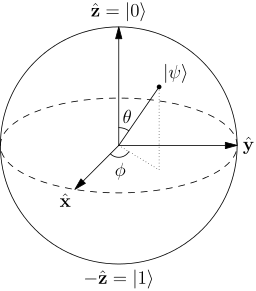
\includegraphics[width=0.4\textwidth]{bloch-sphere.png}
  \caption{The Bloch Sphere representation of a single qubit\cite{Wikipedia}.}
  \label{fig:blochSphere}
  \end{figure}

\section{Survey}
\subsection{The BB84 Protocol}
The BB84 protocol, based on Stephen Wiesner's work on conjugate coding\cite{Wiesner}, was the first QKD scheme to be proposed and is the most common QKD protocol used today. Its security relies on the fact that two non-commuting observables cannot be measured simultaneously. The protocol requires Alice and Bob to select one of two non-orthogonal bases at random when encoding or measuring a polarization state. These bases are the X basis, $\{\ket{0}, \ket{1}\}$, and the Z basis, $\{\ket{+}, \ket{-}\}$, where $\ket{\pm} = \frac{1}{\sqrt{2}}(\ket{0}\pm\ket{1})$. We have seen that $\{\ket{0}, \ket{1}\}$ correspond to the polarization states \ket{\uparrow} and \ket{\rightarrow}, respectively, and that $\{\ket{+}, \ket{-}\}$ correspond to the polarization states \ket{\nwarrow} and \ket{\nearrow}.\\

The BB84 protocol is described as follows\cite{BB84}:
\begin{enumerate}
\item Alice uses a truly random number generator to obtain $(4 + \delta)n$ random classical bits. These bits form the 'raw key', and a subset of the raw key will form the final key shared between Alice and Bob.
\item Alice encodes each bit of her random classical bit string in the polarization state of a photon, according to the following strategy:
  \begin{itemize}
  \item If Alice wishes to send a ``0'', she sends the \ket{0} state in either the X basis (\ket{\uparrow}) or the Z basis (\ket{\nwarrow})  with 50\% probability.
  \item If Alice wishes to send a ``1'', she sends the \ket{1} state in either the X basis (\ket{\rightarrow}) or the Z basis (\ket{\nearrow}) with 50\% probability.
  \end{itemize}
\item Alice sends each polarized photon one at a time over a quantum channel to Bob, who measures each using a birefringent crystal. For each qubit, he randomly chooses to orient his crystal to measure in either the X or the Z basis. If Alice and Bob choose the same basis for encoding and decoding, Bob will measure Alice's original bit value, assuming no channel noise or eavesdropping. Otherwise, his measurement result will be completely uncorrelated with Alice's original bit (see Appendix A2).
\item After measuring the final qubit from Alice, Bob uses an authenticated classical channel to announce his chosen basis for each qubit (but keeping his measured result secret). After Bob has made his announcment, Alice reveals the bases she used to encode the sequence and the two parties discard any bits where they chose differently. In the absence of external noise, the resulting 'sifted' key shared by Alice and Bob must be identical.
\item Alice and Bob agree to announce and then discard a subset of their sifted keys to test for the presence of an eavesdropper. We will show that each time Eve measures a qubit as it travels from Alice to Bob, she will disturb the key in a detectable way with 25\% probability. If Alice and Bob publicly disclose N bits from their sifted keys, they will be able to detect Eve with probability $1 - \frac{3}{4}^N$. Thus, assuming a large enough N it will be extremely unlikely for an eavesdropper to remain undetected.\\
\end{enumerate}

\begin{table}[h]
\caption{BB84 Example Run (without Eve)}
\begin{center}
  \begin{tabular}{|l|c c c c c c c c|}
    \hline
    A's random bits & 1 & 0 & 1 & 0 & 0 & 1 & 1 & 0 \\
    A's bases       & X & Z & Z & Z & X & X & Z & X\\
    Qubits sent & $\rightarrow$ & $\nwarrow$ & $\nearrow$ & $\nwarrow$ & $\uparrow$ & $\rightarrow$ & $\nearrow$ & $\uparrow$ \\
    B's bases         & X & X & Z & X & Z & Z & Z & X \\
    B's results       & 1 & 1 & 1 & 0 & 1 & 0 & 1 & 0 \\
    \hline
    A's key        & 1 & - & 1 & - & - & - & 1 & 0 \\
    B's key        & 1 & - & 1 & - & - & - & 1 & 0 \\
    \hline
  \end{tabular}
\end{center}
\end{table}

Eve wishes to obtain information about Alice's qubits without being detected. In Section II, it was demonstrated that the No-Cloning Theorem prohibits Eve from making a copy of each qubit to measure later. Assume instead that Eve uses an ancillary register (hence 'ancilla') prepared in a standard state \ket{u} to interact with the non-orthogonal states \ket{\psi} and \ket{\phi}. Her goal is to distinguish between \ket{\psi} and \ket{\phi} without disturbing either state and revealing her actions. Assuming this is possible, in the first case Eve obtains
\begin{equation*}
  \begin{split}
    &\ket{\psi}\ket{u}\rightarrow\ket{\psi}\ket{v} \\
    &\ket{\phi}\ket{u}\rightarrow\ket{\phi}\ket{v'}.
  \end{split}
\end{equation*}
To distinguish between the two states, \ket{v} and \ket{v'} must be different. However, we can show that
\begin{equation*}
  \begin{split}
    \ip{v}{v'}\ip{\psi}{\phi}&=\ip{u}{u}\ip{\psi}{\phi} \\
    \ip{v}{v'}&=\ip{u}{u}=1
  \end{split}
\end{equation*}
since inner products are preserved under unitary transformations\cite{Nielsen}. Thus, it must be the case that distinguishing between two non-orthogonal states necessarily disturbs one of them.\\

Because of these limitations, Eve must resort to an intercept-resend strategy that will introduce bit flip errors in Bob's sifted key with high probability. Eve intercepts each of Alice's photons as they travel along the quantum channel to Bob. She measures each photon randomly in either the X or Z basis and records the result. In an attempt to disguise her interference, she re-encodes her result in her chosen basis and forwards the new photon to Bob. As demonstrated for Bob, 50\% of the time Eve and Alice will choose different bases and their bit values will be completely uncorrelated. If this is the case, Eve has a 50\% chance of encoding her result such that Alice, Bob, and Eve all share the same value. By employing this strategy, Eve is able to gain information about 50\% of the key. However, for each photon she measures, she has a 25\% probability of introducing a bit-flip error and revealing her actions.\\

In practice, however, bit-flip errors ofter occur naturally due to imperfections in the quantum channel. One bit-flip error is not sufficient for Alice and Bob to distinguish between channel noise and eavesdropping. Instead, they must estimate a Quantum Bit Error Rate (QBER) for the channel to compare to their measured error rate. If the measured error rate deviates significantly from the QBER, Alice and Bob simply abort the protocol and try again on another channel. Thus, Eve must only measure a small subset of the $(4+\delta)n$ qubits to minimize the number of errors she introduces.\\

\begin{table}[h]
\caption{BB84 Example Run (with Eve)}
\begin{center}
  \begin{tabular}{|l|c c c c c c c c|}
    \hline
    A's random bits & 0 & 1 & 1 & 0 & 1 & 1 & 1 & 0\\
    A's bases       & X & Z & Z & X & Z & X & X & X\\
    Qubits sent & $\uparrow$ & $\nearrow$ & $\nearrow$ & $\uparrow$ & $\nearrow$ & $\rightarrow$ & $\rightarrow$ & $\uparrow$\\
    E's bases       & Z & Z & X & Z & X & X & Z & Z\\
    E's results     & 1 & 1 & 1 & 0 & 0 & 1 & 0 & 0\\
    New qubits  & $\nearrow$ & $\nearrow$ & $\rightarrow$ & $\nwarrow$ & $\uparrow$ & $\rightarrow$ & $\nwarrow$ & $\nwarrow$\\
    B's bases       & X & X & Z & X & Z & Z & X & X\\
    B's results     & 0 & 1 & 0 & 1 & 0 & 1 & 0 & 0\\
    \hline
    A's key         & 0 & - & 1 & 0 & 1 & - & 1 & 0\\
    B's key         & 0 & - & 0 & 1 & 0 & - & 0 & 0\\
    \hline
  \end{tabular}
\end{center}
\end{table}

It is easy to see that the four states used in this protocol lie in the same plane in the Bloch sphere. The basis states of the X basis correspond to the North and South poles of the Bloch sphere, and the basis states of the Z basis correspond to the East-West antipodal points\cite{Williams}. However, there are two more non-orthogonal states perpendicular to this plane which are not used in BB84. Increasing the number of bases from two to three leads to the 'six-state protocol', a generalization of BB84 which can be shown to reduce the information obtainable by an attacker (see Appendix A4).\\

\subsection{Post-Processing}
In the real world, assuming an imperfect channel, Alice's and Bob's sifted keys will contain errors with high probability, even in the absence of eavesdroppers. To correct these errors and guarantee their keys are identical they will need to perform some classical error reconciliation protocol. The CASCADE protocol\cite{Salvail} allows Alice and Bob to correct errors in their keys over a public classical channel without disclosing significant information about their keys. Using their sacrificed bits from step $(5)$ of BB84, Alice and Bob can establish $p*$, an estimate of the probability a bit is flipped in their sifted keys. They then proceed with the CASCADE protocol as follows\cite{Williams}:
\begin{enumerate}
\item Alice and Bob choose a block size based on $p*$ and segment their keys $K_A$ and $K_B$.
\item They perform their own parity measurement on each block and announce the results.
\item If the parity values for a given block differ, that block must contain an odd number of bit-flip errors. If this is the case, Alice and Bob perform the following recursive algorithm\cite{Salvail}:
  \begin{enumerate}
  \item Alice sends Bob the parity of the first half of her block.
  \item Bob determines which half contains the odd number of errors by comparing his parity with Alice's.
  \item This process is repeated until the error is found, then Bob flips his value to correct.
  \end{enumerate}
\item Alice and Bob repeat the protocol until they are confident that no errors remain.
\end{enumerate}

After a sufficient number of applications, the CASCADE protocol will guarantee that Alice and Bob share the same key. Although this protocol is relatively simple to implement compared to other error correction schemes, it requires a large amount of communication overhead. Alice and Bob must announce a parity value for each block, and $\log_2 k$ bits for each $k$-bit block with an odd number of errors. For example, if they estimate a QBER of 5\% using 1000-bit keys with $k=15$, they will need to exchange approximately 350 parity values for a single application of CASCADE\cite{Johnson}. An alternative technique using sparce matrices called Low Density Parity Check (LDPC) codes\cite{Gallager} can be used to provide the same result with much lower overhead\cite{MacKay}.\\

After error reconciliation, it is still possible for an eavesdropper to have obtained a small amount of information about the shared key. This information can come from the initial transmission of photons, assuming Eve chose a small enough $N$ to avoid detection, or from the parities exchanged during error reconciliation. Alice and Bob should now apply a classical privacy amplification algorithm to generate a shorter, secure key that Eve has no information about.\\

Privacy amplification is typically accomplished using an authenticated two-universal hash function. A hash function $f$ is two-universal if for any distinct $x_a,x_b\in X$, the random variables $f(x_a)$ and $f(x_b)$ are independent and uniformly distributed\cite{Renner}. We can determine the amount of information leaked by measuring the uncertainty in Alice's and Bob's key strings. The Shannon entropy, $H(X)$, measures the uncertainty of a random variable $X$. Let $X$ and $Y$ be random variables over the finite sets $\{0,1\}^n$ and $\{0,1\}^r$. Then the Shannon entropy of $X$, $H(X)$, and the Shannon entropy of $X$ conditioned on $Y$, $H(X|Y)$, are defined as
\begin{equation*}
  \begin{split}
    H(X) = -\sum_{x\in X}Pr[X = x&]\log_2 Pr[X = x],\\
    H(X|Y) = -\sum_{x\in X}Pr[X = x|Y =& y]\log_2 Pr[X = x|Y = y].\\
  \end{split}
\end{equation*}
The mutual information\cite{Ribeiro} between two random variables $X$ and $Y$, $I(X,Y)$ is defined as \[ I(X,Y) = H(X) - H(X|Y). \]Assume Alice's original bits form string $X$, Bob's measurement results form string $Y$, and $Z$ represents the information known to Eve. After Alice and Bob input their matching keys into an authenticated two-universal hash function, we get the result \[ I(X,Y)\approx 0. \]\\

\subsection{The B92 Protocol}
In 1992, Bennett\cite{B92} showed that only two non-orthogonal states are necessary to perform quantum key distribution, as opposed to the four required in BB84 (\ket{\uparrow}, \ket{\rightarrow}, \ket{\nwarrow}, and \ket{\nearrow}). This is accomplished by replacing the birefringent crystals used in BB84 with polarization filters, which transmit or absorb photons probabilistically based on the angle between the axis of measurement and the axis of polarization. For example, a vertically polarized photon measured with a vertical polarization filter will be transmitted with 100\% probability, while a horizontally polarized photon will be absorbed by the same filter with 100\% probability. A photon polarized at $\pm45\degree$ will be either transmitted or absorbed with 50\% probability. It is important to note that the polarization axis of a transmitted photon is necessarily aligned with the axis of the filter, and thus the original state information is lost when measured.\\

The B92 protocol is described as follows\cite{B92}:
\begin{enumerate}
\item Alice uses a truly random number generator to obtain a long string of random classical bits. As in BB84, these bits form Alice's raw key.
\item Alice encodes each bit of her random classical bit string in the polarization state of a photon, according to the following strategy:
  \begin{itemize}
  \item If Alice wishes to send a ``0'', she sends the \ket{0} state in the X basis, \ket{\uparrow}.
  \item If Alice wishes to send a ``1'', she sends the \ket{0} state in the Z basis, \ket{\nwarrow}.
  \end{itemize}
\item Bob randomly chooses one of two polarization filters to measure each photon with. The first possible polarizer is oriented such that it transmits the state \ket{\nearrow} and blocks the state\ket{\nwarrow}. If Alice's original bit value was ``1'', her qubit will be absorbed with 100\% probability. Otherwise it will be either transmitted or absorbed with 50\% probability. Thus this filter can only test whether Alice sent a ``0''. The other possible filter transmits the state \ket{\rightarrow} and absorbs the state \ket{\uparrow}, effectively testing for the value ``1''. Thus, Bob will only obtain a measurement result for 25\% of the photons sent by Alice. If Bob does obtain a result, however, he knows that his bit value for that photon is perfectly correlated with Alice's (see Appendix A3).
\item After measuring the final qubit from Alice, Bob uses an authenticated classical channel to announce the photons for which he obtained a measurement result (but keeping his measured result secret). Since Alice knows the original bit values she sent, she can figure out the results of Bob's measurements and derive the same shared key as Bob.
\item As in BB84, Alice and Bob attempt to detect any eavesdropping by comparing and discarding a subset of their sifted keys. They also monitor the number of qubits lost during the protocol to prevent against an attack specific to B92.\\
\end{enumerate}
\begin{table}[h]
  \caption{Example run of B92 (without Eve)}
  \begin{center}
    \begin{tabular}{|l|c c c c c c c c|}
      \hline
      A's random bits & 1 & 0 & 0 & 0 & 1 & 0 & 1 & 1\\
      Qubits sent & $\nwarrow$ & $\uparrow$ & $\uparrow$ & $\uparrow$ & $\nwarrow$ & $\uparrow$ & $\nwarrow$ & $\nwarrow$\\
      B tests for     & 1 & 1 & 0 & 0 & 1 & 1 & 1 & 0\\
      B's results     & 1 & - & - & 0 & - & - & 1 & -\\
      \hline
      A's key         & 1 & - & - & 0 & - & - & 1 & -\\
      B's key         & 1 & - & - & 0 & - & - & 1 & -\\
      \hline
    \end{tabular}
  \end{center}
\end{table}

While B92 requires fewer states than BB84, making it easier to implement, the fact that most of the photons are discarded leaves it vulnerable to a subtle eavesdropping strategy. While we have demonstrated that distinguishing between non-orthogonal states is impossible, Eve can simply discard failed attempts to determine Alice's raw key with 100\% accuracy\cite{Williams}. The only way for Alice and Bob to detect this type of attack is to establish an expected qubit loss rate for the channel and compare it with the actual loss rate. However, if Eve controls the quantum channel while Alice and Bob perform their setup, she may be able to manipulate the expected loss rate and avoid detection. As a result of this vulnerability, B92 is rarely implemented in real-world QKD systems.\\

\subsection{The E91 Protocol}
The E91 protocol, developed by Artur Ekert\cite{E91}, uses quantum entanglement to provide a guarantee of security. To provide context to this protocol, we must examine two assumptions made in 1935 by Einstein, Podolski, and Rosen\cite{EPR}:
\begin{itemize}
\item Reality: The value of a measurement exists even before the measurement takes place.
\item Locality: The measurement result for one object has no influence on the reality of distant objects.
\end{itemize}
In 1964, Bell demonstrated that measuring the state of one entangled particle immediately collapses the state of its complement, regardless of the distance between them\cite{Bell}. This defies the theory of local realism described by EPR and represents the incompatibility between classical and quantum mechanics.\\

The E91 protocol is described as follows\cite{E91}:
\begin{enumerate}
\item Alice and Bob acquire $n$ sets of entangled qubits in the singlet state \[ \frac{1}{\sqrt{2}}(\ket{01} - \ket{10}), \] distributing one qubit from each pair to Alice and the other to Bob. Either party could generate the pairs and send half of the qubits to the other, or they could rely on a trusted third party to generate the entangled pairs.
\item For each qubit, Alice chooses an angle uniformly at random from the set \[ {\phi_i}^A = \{0, \frac{\pi}{8}, \frac{\pi}{4}\}. \]She then rotates the vertical-horizontal basis by her chosen angle around the z-axis and measures the qubit with respect to the new basis. Bob then does the same, instead choosing his angle from the set \[ {\phi_j}^B = \{0, \frac{\pi}{8}, \frac{-\pi}{8}\}. \]
\item If Alice and Bob orient their measurement devices the same way, Bob's result will be perfectly anti-correlated with Alice's. That is, in two of the nine cases, Alice and Bob will always measure opposite bit values and can therefore establish a shared key.
\item The measurement values of qubits where Alice and Bob chose different measurement axes are announced and used to calculate the correlation coefficient of their measurements:
  \begin{equation*}
    \begin{split}
      E({\phi_i}^A, {\phi_j}^B) = &P_{00}({\phi_i}^A,{\phi_j}^B) + P_{11}({\phi_i}^A,{\phi_j}^B)\\
      - &P_{01}({\phi_i}^A,{\phi_j}^B) - P_{10}({\phi_i}^A,{\phi_j}^B),\\
    \end{split}
  \end{equation*}
  where $P_{00}$ represents the probability of Alice and Bob both obtaining 0 as the measurement result.
\item Alice and Bob calculate the quantity
  \begin{equation*}
    \begin{split}
      S = &E({\phi_1}^A,{\phi_2}^B) + E({\phi_1}^A,{\phi_4}^B)\\
      + &E({\phi_3}^A,{\phi_2}^B) - E({\phi_3}^A,{\phi_4}^B),\\
    \end{split}
  \end{equation*}
  composed from the correlation coefficients for which Alice and Bob chose different measurement axes. Bell's Theorem requires that, in the absence of an eavesdropper, $S=-2\sqrt{2}$\cite{Clauser}. If this does not match Alice's and Bob's measurements, then they detect Eve's interference and abort the protocol.\\
\end{enumerate}

\begin{table}[h]
  \caption{Example Run of E91 (without Eve)}
  \begin{center}
    \begin{tabular}{|l|c c c c c c c c c c c c|}
      \hline
      A's bases   & 2 & 2 & 1 & 3 & 1 & 1 & 3 & 1 & 3 & 1 & 1 & 2\\
      B's bases   & 1 & 4 & 1 & 2 & 4 & 1 & 2 & 1 & 2 & 4 & 2 & 2\\
      A's results & 0 & 1 & 1 & 0 & 1 & 0 & 0 & 0 & 1 & 1 & 0 & 0\\
      B's results & 1 & 1 & 0 & 0 & 1 & 1 & 0 & 1 & 0 & 0 & 1 & 1\\
      \hline
      A's key     & - & - & 1 & - & - & 0 & - & 0 & - & - & - & 0\\
      B's key     & - & - & 1 & - & - & 0 & - & 0 & - & - & - & 0\\
      \hline
    \end{tabular}
  \end{center}
\end{table}
The security of the E91 protocol lies in the fact that neither Alice nor Bob generates the key material to send to the other. Instead, the key does not exist until Alice and Bob perform their measurements, meaning Eve cannot perform an intercept-resend attack as in BB84. Any attempt by Eve to substitute her own prepared data for Alice's and Bob's communication is the same as introducing elements of physical reality to the quantum system, bounding S to $-\sqrt{2}\leq S\leq\sqrt{2}$ and thus revealing her actions\cite{Bouwmeester}.\\

\section{Simulations}
Each of the simulations prepared for this project was written in Python 2.7. Each uses the following modules:
\begin{itemize}
\item NumPy for random sampling and bitwise operations
\item PyCrypto for cryptographic random number generation
\item The Quantum Information Toolkit (QIT) to represent and measure quantum states
  \item Nose for unit testing
\end{itemize}
Each simulation accepts a desired key length as well as optional parameters to control eavesdropping or the QBER. It then performs the selected protocol up to the sifting phase and returns the sifted key, or failure in the case that an eavesdropper is detected. The Appendix of this report contains three outputs for the BB84 and B92 protocols:
\begin{itemize}
\item One run with no channel noise and no eavesdropping which yields identical keys.
\item One run with a small amount of channel noise but no eavesdropping, leading to key errors but not an abortion of the protocol.
\item One run with channel noise and eavesdropping, which Alice and Bob detect.
\end{itemize}
The E91 simulation does not simulate an eavesdropper due to the difficulty of implementing Eve's optimal strategy.\\

Three of the eleven unit tests, test\_bb84(), test\_b92(), and test\_e91(), simply perform 20 trials of the appropriate protocol with a desired key size of 2048 bits and assert that a shared key is successfully established. Two of the tests, test\_decodeStateBB84\_probabilistic() and test\_getRandomBits(), are probabilistic and assert that expected probabilities are met for large key sizes. The remaining six tests verify deterministic cases, such as measuring an entangled state along two identical axes of measurement.\\

\section{Conclusion}
Quantum key distribution is one of the most developed ideas quantum computing, as it is one of the only applications of quantum computing with practical implementations in industry. However, classical public-key schemes remain the dominant method of distributing key material in the real world. The advantages of QKD over classical key distribution are immediately apparent, since breaking the security of QKD requires an attacker to violate fundamental physical laws. As technological advances lead to improvements in range and transmission rates, we may see protocols such as BB84 become the standard for key distribution in the near future.\\

Each of the three protocols surveyed has its own advantages and disadvantages relative to the others. The protocol most likely to be adopted on a large scale is BB84, as it is relatively intuitive, easy to implement, and provably secure. The E91 protocol, which relies on entangled particles, provides a similar guarantee of security to BB84 but is not as well-documented or intuitive, making it an unlikely candidate for a QKD standard. E91 shows potential at longer distances, however, as it can be implemented without the use of a noisy quantum channel if Alice and Bob generate their entangled pairs in person and save them until the protocol is performed. B92, while originally celebrated as a more intuitive version of BB84, will likely not see much real-world implementation due to the extra monitoring and precautions it requires.\\

Besides relatively poor range and transmission rates, the largest barrier to adoption for QKD is the difficulty of producing specific quantum states outside of the laboratory. In all protocols, but especially in E91, users will likely be forced to rely on a trusted third party to generate and distribute the necessary qubits. While protocols like BB84 have the potential to replace classical key distribution schemes, significant advances in hardware will be necessary before QKD becomes practical for the average user.\\

\begin{thebibliography}{26}
\bibitem[1]{BB84}
  C. H. Bennett and G. Brassard, ``Quantum Cryptography: Public Key Distribution and Coin Tossing,'' Intl. Conf. on Computers, Systems, \& Signal Processing, 12 Dec. 1984.
\bibitem[2]{B92}
  C. H. Bennett, ``Quantum Cryptography Using Any Two Nonorthogonal States,'' Phys. Rev. Lett., Volume 68, Number 21, 25 May 1992.
\bibitem[3]{E91}
  A. K. Ekert, ``Quantum Cryptography Based on Bell's Theorem,'' Phys. Rev. Lett., Volume 67, Number 6, 5 August 1991.
\bibitem[4]{Rivest}
  R. Rivest, A. Shamir, and L. Adleman, ``On Digital Signatures and Public Key Cryptosystems,'' Commun. Ass. Comp. Mach., Volume 21 (1978) pp. 120-126.
\bibitem[5]{Rosing}
  M Rosing, ``Implementing Elliptic Curve Cryptography,'' Manning Publications, Greenwich (1999) ISBN 1-884777-69-4.
\bibitem[6]{Weisstein}
  E. W. Weisstein, ``RSA-640 Factored,'' MathWorld Headline News, 8th November (2005),
  http://mathworld.wolfram.com/news/2005-11-08/rsa-640/.
\bibitem[7]{Shor}
  P. Shor, ``Polynomial-time Algorithms for Prime Factorization and Discrete Logarithms on a Quantum Computer,'' Siam Journal on Computing, Volume 26, Issue 5 (1997) pp. 1484-1509.
\bibitem[8]{Heninger}
  N. Heninger, Z. Durumeric, E. Wustrow, J. A. Halderman, ``Mining Your Ps and Qs: Detection of Widespread Weak Keys in Network Devices,'' Proc. 21st USENIX Security Symposium, Aug. 2012.
\bibitem[9]{Jun}
  B. Jun and P. Kocher, ``The Intel Random Number Generator,'' Cryptography Research, Inc. white paper prepared for Intel Corp., 22 Apr. 1999.
\bibitem[10]{Kaye}
  P. Kaye, R. LaFlamme, M. Mosca, \textit{An Introduction to Quantum Computing}, Oxford UP, 2010. Print. ISBN 978-0-19-857049-3.
\bibitem[11]{Wimmel}
  H. Wimmel, \textit{Quantum Physics \& Observed Reality: A Critical Interpretation of Quantum Mechanics}, World Scientific, 1992. Print. ISBN 981-02-1010-8.
\bibitem[12]{Williams}
  C. Williams, \textit{Explorations in Quantum Computing}, Springer, 2011. Print. ISBN 978-1-84628-886-9.
\bibitem[13]{Wootters}
  W. K. Wootters and W. H. Zurek, ``A Single Quantum Cannot Be Cloned,'' Nature, Volume 299, pp. 802-803. 28 Oct. 1982.
\bibitem[14]{Wikipedia}
  Wikipedia, the free encyclopedia, ``Bloch Sphere,''
  URL: upload.wikimedia.org/wikipedia/commons/thumb/f/f4/Bloch\_Sphere.svg/256px-Bloch\_Sphere.svg.png
\bibitem[15]{Wiesner}
  S. Wiesner, ``Conjugate Coding,'' SIGACT News, Volume 15, Number 1, Jan. 1982.
\bibitem[16]{Nielsen}
  M. Nielsen and I. Chuang, ``Quantum Computation and Quantum Information,'' Cambridge UP, 2015. Print.
\bibitem[17]{Salvail}
  G. Brassard and L. Salvail, ``Secret-Key Reconciliation by Public Discussion,'' Proc. Eurocrypt 93 Workshop on the Theory and Application of Cryptographic Techniques, pp. 410-423, 23-27 May 1993.
\bibitem[18]{Johnson}
  J. Johnson, ``An Analysis of Error Reconciliation Protocols for Use in Quantum Key Distribution,'' Master's Thesis, Air Force Institute of Technology, Feb. 2012.
\bibitem[19]{Gallager}
  R. Gallager, ``Low-Density Parity-Check Codes,'' Doctoral Thesis, Massachusetts Institute of Technology, 1960.
\bibitem[20]{MacKay}
  D. J. MacKay, ``Good Error-Correcting Codes Based on Very Sparse Matrices,'' IEEE Transactions on Information Theory, Jan. 1999.
\bibitem[21]{Renner}
  R. Renner, R. K\"onig, ``Universally Composable Privacy Amplification Against Quantum Adversaries,'' In: Kilian J (eds) Theory of Cryptography, TCC 2005. Lecture Notes in Computer Science, Volume 3378. Springer, Berlin, Heidelberg.
\bibitem[22]{Ribeiro}
  A. S. Ribeiro, S. A. Kauffman, J. Lloyd-Price, B. Samuelsson, and J. Socolar, ``Mutual Information in Random Boolean Models of Regulatory Networks,'' Physical Review E, 77(1):011901, 2008.
\bibitem[23]{EPR}
  A. Einstein, B. Podolski, N. Rosen, ``Can Quantum-Mechanical Description of Physical Reality be Considered Complete?'' Phys. Rev. 47 (10), pp. 777-780. 1935.
\bibitem[24]{Bell}
  J. S. Bell, ``On the Einstein-Podolski-Rosen Paradox,'' Physics. 1, pp. 195-200. 1964.
\bibitem[25]{Clauser}
  J. F. Clauser, M. A. Horne, A. Shimony, R. A. Holt, ``Proposed Experiment to Test Local Hidden-Variable Theories,'' Phys. Rev. Lett. 23 (15), pp. 880-884. 1969.
\bibitem[26]{Bouwmeester}
  D. Bouwmeester, A. Ekert, A. Zeilinger, ``The Physics of Quantum Information,'' Springer-Verlag, Berlin, 2000.
\end{thebibliography}

\appendix
\section{Appendix A}
\begin{itemize}
\item [A1)] Exercise 12.25: Consider a system with $n$ users, any pair of which would like to be able to communicate privately. Using public key cryptography how many keys are required? Using private key cryptography how many keys are required?
  \begin{itemize}
  \item [a] Using public key cryptography, each user has 2 keys: 1 public and 1 private. Thus there are $2n$ unique keys. Since each of the $n$ users needs a copy of the other $n-1$ public keys plus their private key, there is a total of $n^2$ key copies required.
  \item [b] Using private key cryptography, each unique pair of users requires a unique shared key. This can be visualized as a complete graph, with $n$ nodes representing users. We know that for a complete graph with $n$ nodes, there are $\frac{n(n-1)}{2}$ edges, so there must be $\frac{n(n-1)}{2}$ keys.
  \end{itemize}
\item [A2)] Exercise 12.26: Let $a_k, a'_k$ be Alice's and Bob's classical bit values associated with qubit \ket{\psi_{{a_k}{b_k}}} in the BB84 protocol, and let $b_k, b'_k$ be Alice and Bob's randomly chosen bases. Assuming a noiseless channel with no eavesdropping, show that when $b'_k\neq b_k$, $a'_k$ is random and completely uncorrelated with $a_k$. But when $b'_k=b_k$, $a'_=a_k$.
  \begin{itemize}
  \item [a] When $b'_k\neq b_k$, Alice's and Bob's bases are offset by 45\degree. This is equivalent to measuring the state \[ \frac{1}{\sqrt{2}}(\ket{0}\pm\ket{1}) \]in the computational basis, which yields either ``0'' or ``1'' with 50\% probability. Thus, in this case $a'_k$ is random and completely uncorrelated with $a_k$.
  \item [b] When $b'_k= b_k$, Alice's and Bob's bases are identical. Since Alice's encoding is a pure state with probability amplitude of $1$, Bob's measurement will deterministically return $a'_k=a_k$.
  \end{itemize}
\item [A3)] Exercise 12.28: Let $a$ represent Alice's raw key, $a'$ represent Bob's chosen filter orientation, and $b$ represent Bob's measurement result for each qubit in the B92 protocol. Show that when $b=1$, then $a$ and $a'$ are perfectly correlated with each other.
  \begin{itemize}
  \item [a] Consider the case where $a=a'=0$: Alice sends Bob the \ket{0} state, which he measures in the X basis, yielding ``0'' with 100\% probability. If $a=a'=1$, Alice sends Bob the ``0'' state in the Z basis, $\frac{1}{\sqrt{2}}(\ket{0}+\ket{1})$, and Bob measures in the Z basis to obtain ``0'' with 100\% probability. Bob can only obtain ``1'' when $a\neq a'$, and in this case he measures ``1'' with 50\% probability. However, if he measures ``1'' he knows that his $a'$ is necessarily $1-a$ and thus $a$ and $a'$ are perfectly correlated.
  \end{itemize}
\item [A4)] Exercise 12.29: Give a protocol using six states, the eigenstates of X, Y, and Z, and argue why it is also secure. Discuss the sensitivity of this protocol to noise and eavesdropping, in comparison with that of BB84 and B92.
  \begin{itemize}
  \item [a] The three bases in a six-state protocol would be the X basis, $\{\ket{0},\ket{1}\}$, the Z basis, $\{\frac{1}{\sqrt{2}}(\ket{0}\pm\ket{1})\}$, and the Y basis, $\{\frac{1}{\sqrt{2}}(\ket{0}\pm\iu\ket{1})\}$. In this scheme, Alice and Bob have a $\frac{1}{3}$ probability of choosing the same basis instead of the $\frac{1}{2}$ probability in BB84. This means that more qubits will be discarded during sifting, but it also increases the likelihood of detecting Eve each time she measures a quantum state. Eve now has a $\frac{2}{3}$ probability of choosing the wrong basis, and when this occurs she has a $\frac{1}{2}$ probability of re-encoding the wrong value. Thus, if she measures every qubit, the QBER for the six-state protocol will be 33\% instead of the 25\% for BB84.
  \end{itemize}
\end{itemize}

% that's all folks
\end{document}
